% Appendix: Figure 8 Investigation - Sentiment Negation Circuits
% This appendix documents the full investigation of AND-gate circuits in fw-medium

\section{Sentiment Negation Circuit Investigation}
\label{app:figure8_investigation}

This appendix presents our detailed investigation of AND-gate circuits in bilinear transformers.

\subsection{SAE Availability Investigation}
\label{app:sae_availability}

We investigated the publicly available SAEs on HuggingFace to determine reproducibility constraints.

\textbf{ts-medium-scope} (paper's ``ts-tiny'', 6 layers):
\begin{itemize}[leftmargin=*,topsep=0pt,itemsep=0pt]
    \item Layers 0--4: Only \texttt{mlp-out}, \texttt{resid-mid}, \texttt{resid-pre} SAEs
    \item Layer 5: \texttt{mlp-in} and \texttt{mlp-out} available
    \item \textbf{Critical: No \texttt{mlp-in} SAE at layer 4}---the layer used in the paper's Figure 8
\end{itemize}

\textbf{fw-medium-scope} (16 layers):
\begin{itemize}[leftmargin=*,topsep=0pt,itemsep=0pt]
    \item All layers 0--15: \texttt{mlp-in} and \texttt{mlp-out} at 8$\times$ expansion
    \item Layer 12: Additional v0--v4 training-time variants at 16$\times$ expansion
\end{itemize}

Since Figure 8 analysis requires \emph{both} \texttt{mlp-in} and \texttt{mlp-out} SAEs (for the Tracer class), the paper's Figure 8 (ts-tiny, layer 4) cannot be reproduced with public artifacts.
We therefore use fw-medium (layer 7, expansion 8) which has both SAE types available.
The paper's tutorial also uses fw-medium with features 3834/751, confirming this is a valid alternative.

\subsection{AND-gate Circuit Analysis}

The following analysis uses fw-medium (16 layers, 335M parameters, trained on FineWeb-EDU) with layer 7 SAEs at 8$\times$ expansion (8,192 output features).

\subsubsection{AND-gate Circuit Definition}
An AND-gate circuit is characterized by an output SAE feature whose activation depends on the \emph{conjunction} of inputs from two semantically distinct clusters.
Mathematically, for output feature $c$, the activation is:
\begin{equation}
z_c(x) = x^\top Q_c x \approx \lambda_1 (v_1^\top x)^2 + \lambda_2 (v_2^\top x)^2
\end{equation}
where $Q_c$ is the interaction matrix, and $v_1, v_2$ are the dominant eigenvectors.

Strong AND-gate behavior requires:
\begin{enumerate}
    \item \textbf{Dominant rank-2 structure}: The top two eigenvalues capture most of the interaction.
    \item \textbf{Opposing eigenvalue signs}: $\lambda_1$ and $\lambda_2$ have opposite signs, creating cancellation when only one cluster is present.
    \item \textbf{Clear cluster separation}: Input features project distinctly onto $v_1$ and $v_2$.
\end{enumerate}

\subsubsection{AND-score Metric}
We define an ``AND-score'' to quantify circuit strength:
\begin{equation}
\text{AND-score} = \frac{|\lambda_1|}{|\lambda_1| + |\lambda_2|} \cdot \mathbf{1}[\text{sign}(\lambda_1) \neq \text{sign}(\lambda_2)]
\end{equation}
Higher scores indicate stronger AND-gate behavior (score $\in [0, 1]$).

\subsubsection{Search Procedure}
We analyzed all 8,192 output features in fw-medium layer 7:
\begin{enumerate}
    \item Computed the interaction matrix $Q_c$ for each feature $c$
    \item Performed eigendecomposition: $Q_c = \sum_j \lambda_j v_j v_j^\top$
    \item Computed AND-score from top eigenvalues
    \item Ranked features by AND-score
    \item Analyzed top circuits for semantic interpretation
\end{enumerate}

\subsection{Results: Feature 3834 vs Feature 751}

\subsubsection{Tutorial Feature 3834}
Feature 3834 (used in the paper's tutorial) encodes ``not-good'' contexts with weaker AND-gate structure:
diffuse eigenvalue spectrum and less distinct cluster separation.

\subsubsection{Best Circuit: Feature 751}
Our search identified feature 751 as having the strongest AND-gate structure (Table~\ref{tab:app_circuit_comparison}).

\begin{figure}[H]
    \centering
    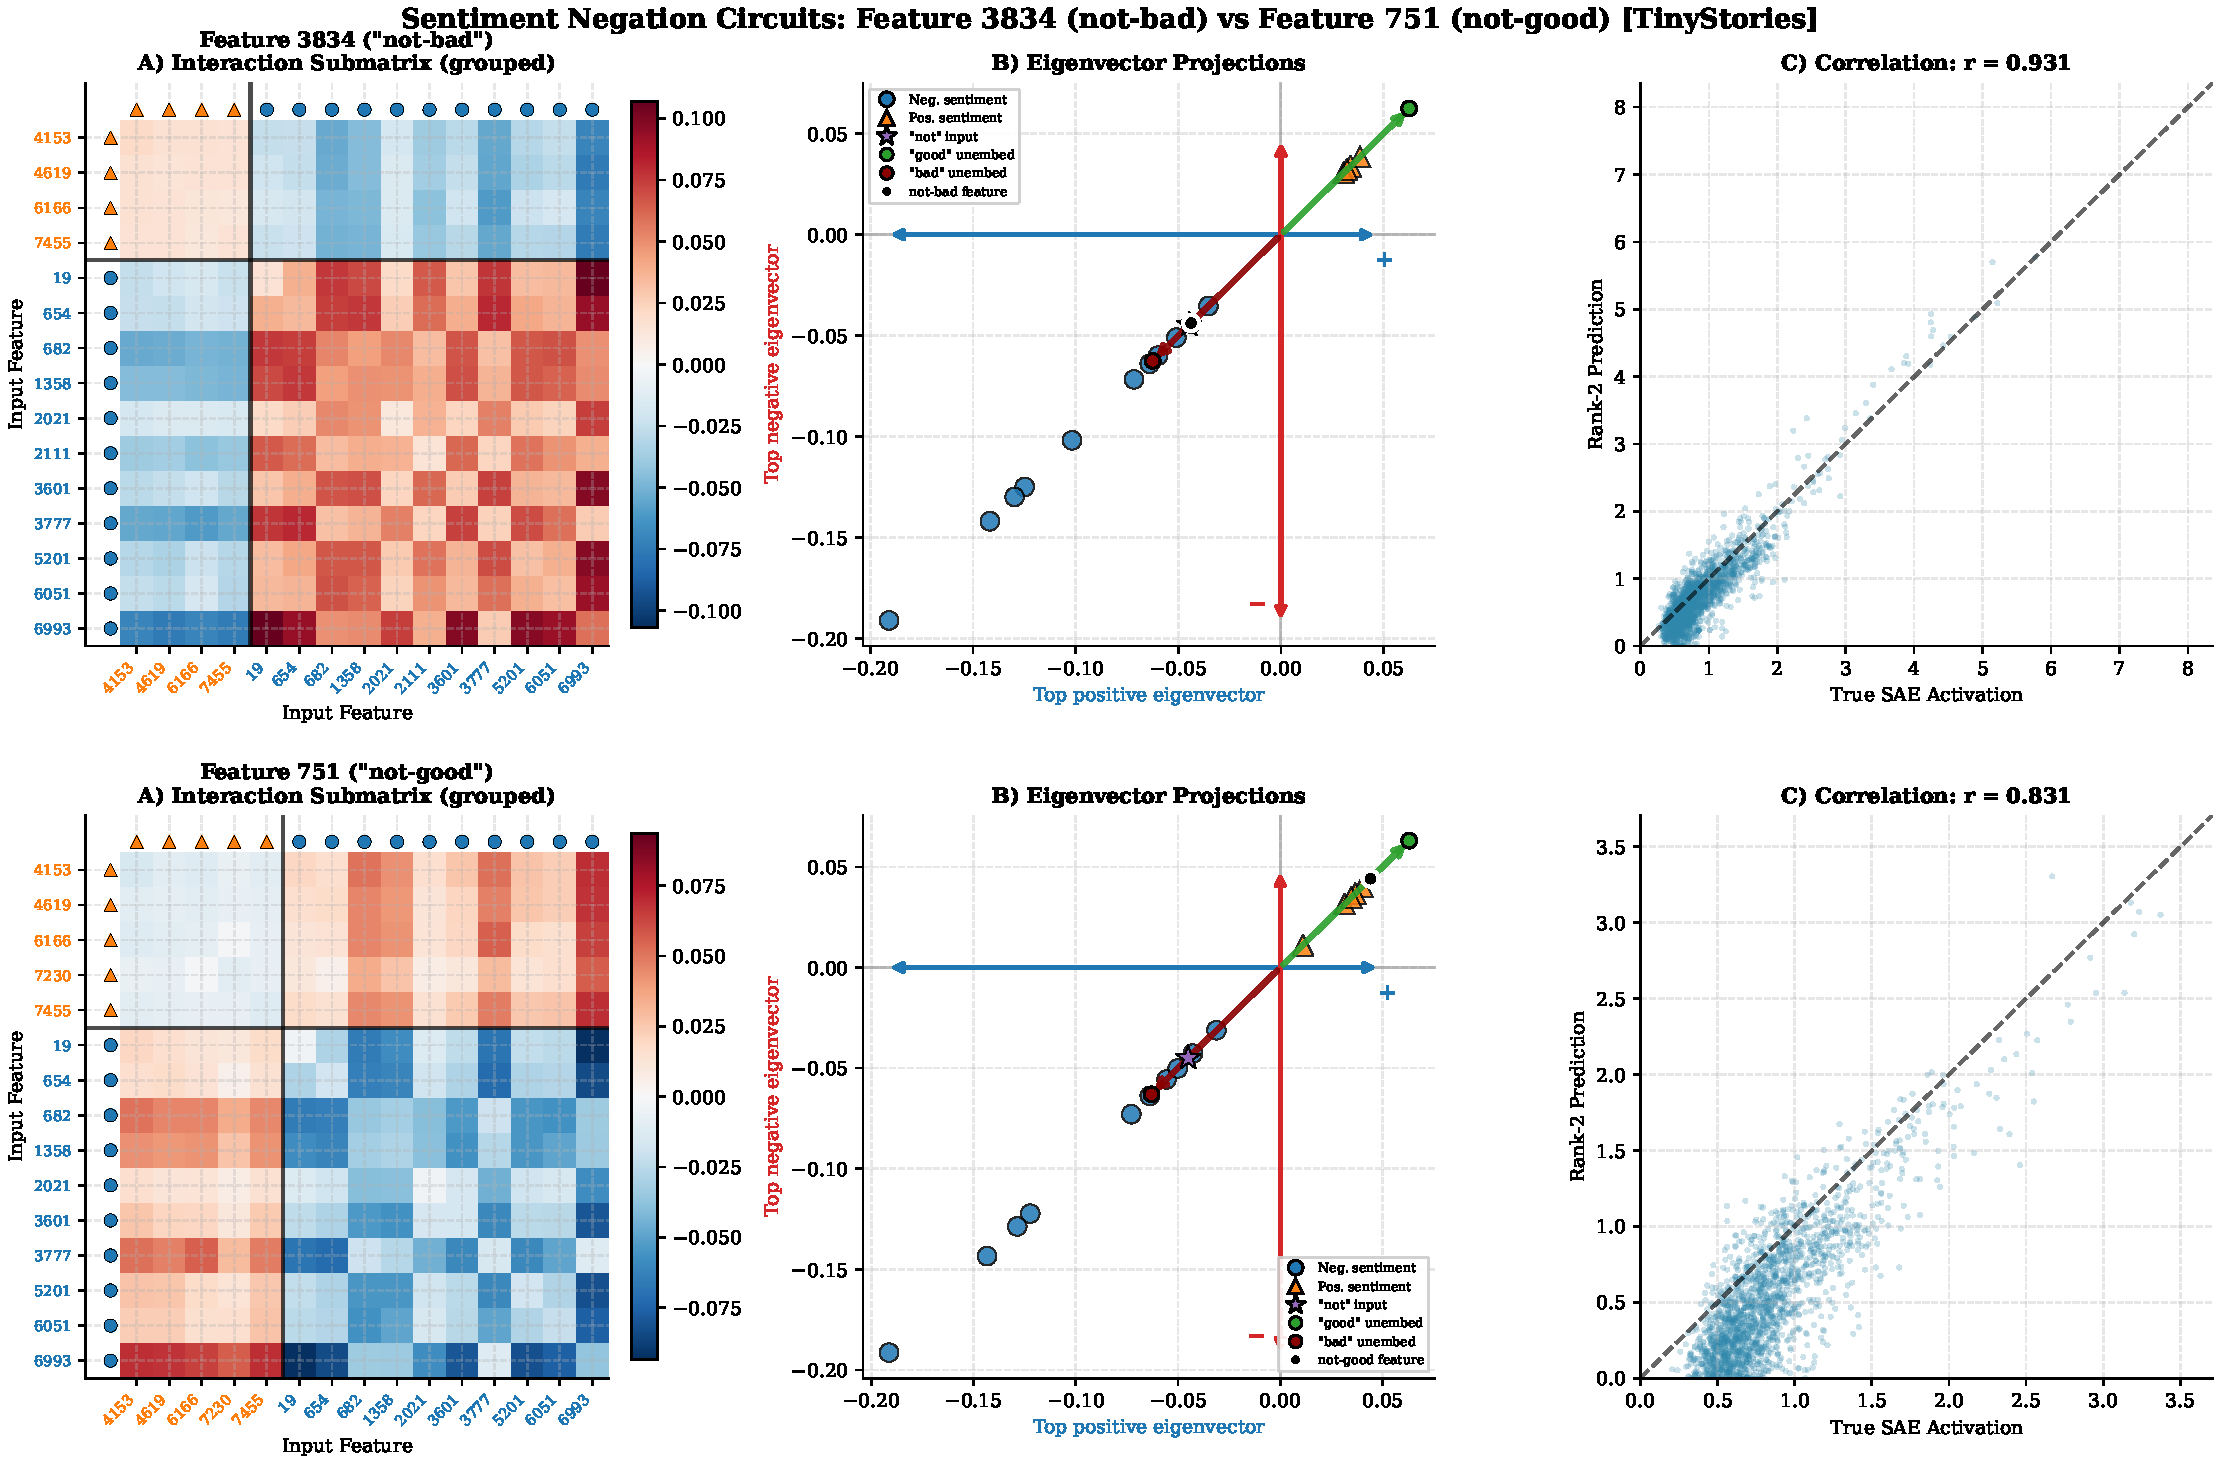
\includegraphics[width=\linewidth]{figures/language/figure_8_final.pdf}
    \caption{AND-gate circuit comparison (TinyStories evaluation).
    \textbf{Top}: Feature 3834 (tutorial) encodes ``not-good'' contexts ($r = 0.93$).
    \textbf{Bottom}: Feature 751 encodes ``not-bad'' contexts ($r = 0.83$).
    The eigenvector projections (middle) separate clusters along opposite axes due to opposing eigenvalues.}
    \label{fig:app_figure8_comparison}
\end{figure}

\subsection{Semantic Interpretation of Feature 751}

The input clusters have clear semantic content based on token analysis:

\textbf{Positive cluster} (3 features: 5212, 7655, 253):
\begin{itemize}
    \item Tokens: ``wonderful'', ``excellent'', ``fortunate'', ``beautiful'', ``amazing''
    \item Semantics: Positive sentiment/quality descriptors
\end{itemize}

\textbf{Negative cluster} (12 features):
\begin{itemize}
    \item Feature 5201: ``horrible'', ``bad'', ``terrible''
    \item Feature 3601: ``problems'', ``illness'', ``disease''
    \item Feature 6051: ``excessive'', ``unfair'', ``wrong''
    \item Feature 6921: ``no'', ``minimal'', ``neither''
    \item Feature 1003: ``reduce'', ``prevent'', ``eliminate''
\end{itemize}

\textbf{Circuit function:} Feature 751 detects contexts where negative concepts appear \emph{without} positive modulation.
The AND-gate structure arises because:
\begin{enumerate}
    \item The top eigenvalue (negative) suppresses activation when positive cluster projects onto $v_1$
    \item The second eigenvalue (positive) activates when negative cluster projects onto $v_2$
    \item When both clusters are present, the opposing signs cause partial cancellation
\end{enumerate}

This confirms the mechanism: high activation requires negative concepts \emph{without} positive sentiment, consistent with a ``problematic situation'' detector.

\subsection{Linear Subspace Structure}
\label{app:linear_subspace}

Following the tutorial methodology, we compute cosine similarity between SAE decoder directions for the top output features with high eigenvalues.
Features 3834 and 751 have cosine similarity $-0.16$---weakly negative, which the tutorial calls a ``somewhat linear subspace.''
Note that $-0.16$ is closer to orthogonal than anti-parallel; the features are \emph{semantic} opposites (not-good vs.\ not-bad) rather than geometrically opposing.
Semantic interpretation comes from inspecting top-activating tokens: feature 3834 fires on negated positive contexts, while feature 751 fires on negated negative contexts.
The paper's tutorial observes: ``It's not surprising that this forms a linear subspace as the two are opposites.''

\subsection{Cross-Dataset Validation}
\label{app:cross_dataset_fig8}

As additional validation beyond the paper, we test the same circuit on FineWeb-16k (the model's training distribution) in addition to TinyStories.
Figure~\ref{fig:app_figure8_fineweb} shows the results, and Table~\ref{tab:cross_dataset_fig8} provides a quantitative comparison.

\begin{figure}[H]
    \centering
    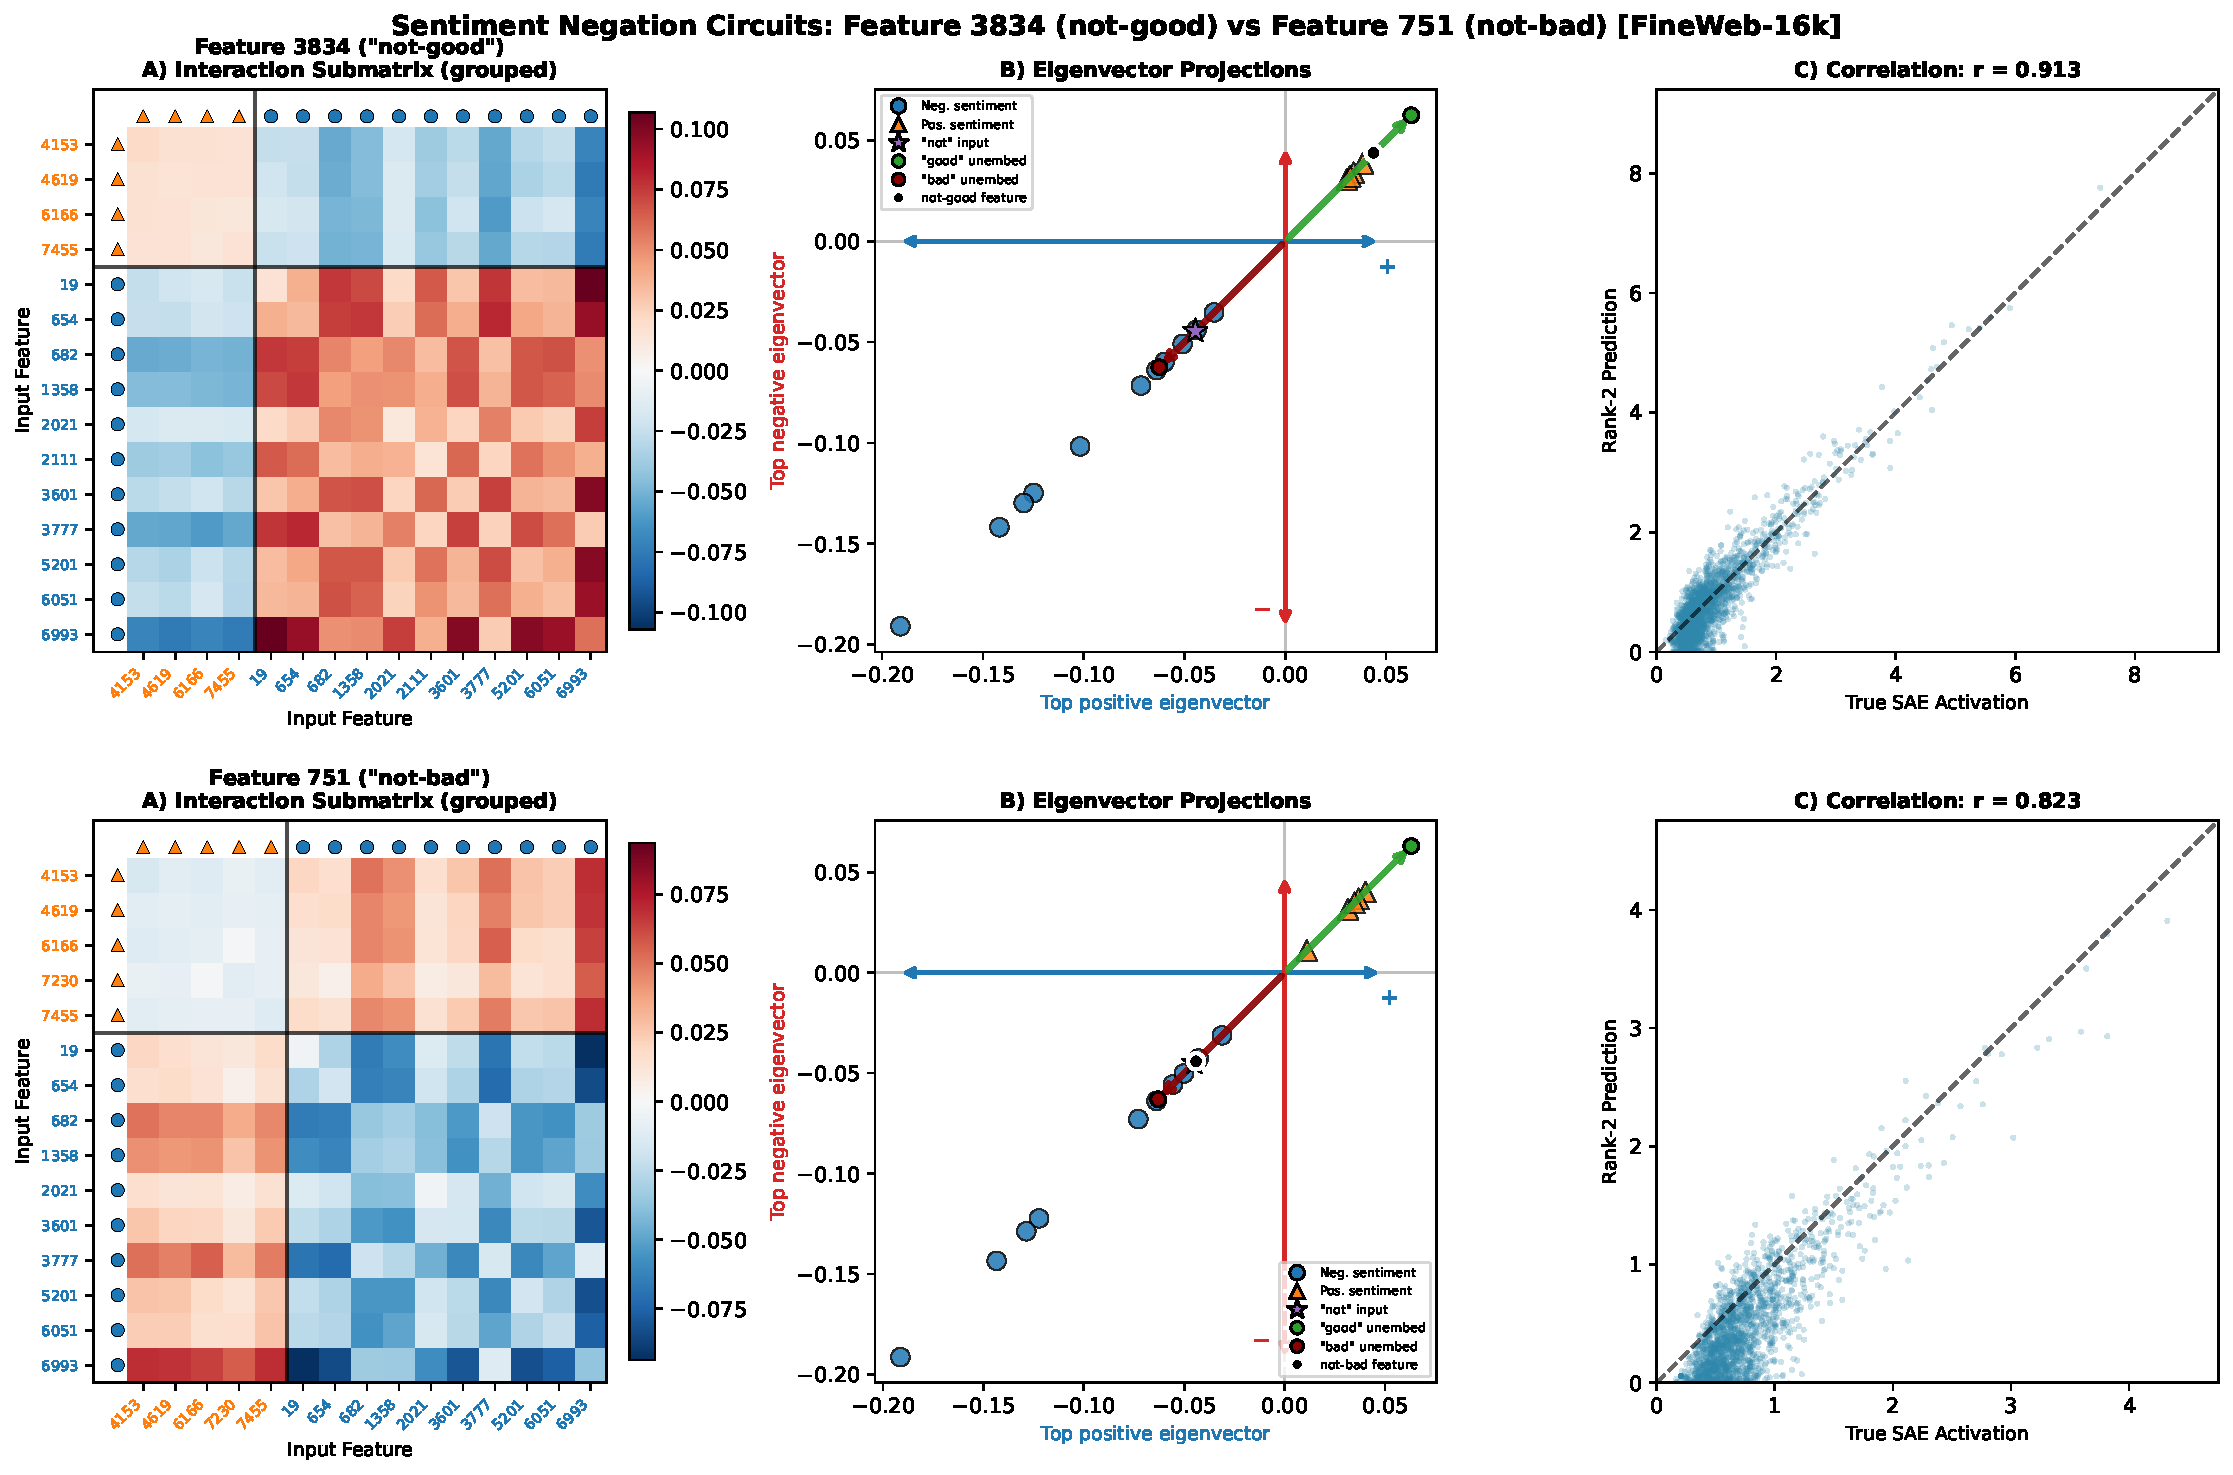
\includegraphics[width=\linewidth]{figures/language/figure_8_final_fineweb16k.pdf}
    \caption{AND-gate circuit on FineWeb-16k (model's training distribution).
    Correlations: 0.91 (feature 3834), 0.82 (feature 751).
    Feature 751 activates more frequently on FineWeb-16k (6,517 vs 2,542 samples), likely due to more ``not-bad'' contexts in educational/scientific text.}
    \label{fig:app_figure8_fineweb}
\end{figure}

\begin{table}[H]
    \centering
    \caption{Cross-dataset comparison of negation circuit correlations.}
    \label{tab:cross_dataset_fig8}
    \begin{tabular}{lccc}
        \toprule
        Feature & TinyStories & FineWeb-16k & $\Delta$ \\
        \midrule
        3834 (not-good) & 0.931 (n=9,719) & 0.913 (n=9,937) & $-0.018$ \\
        751 (not-bad) & 0.831 (n=2,542) & 0.823 (n=6,517) & $-0.008$ \\
        \bottomrule
    \end{tabular}
\end{table}

The correlations remain strong across both datasets, with differences of only 1--2\%.
This demonstrates that the discovered circuit is robust to distribution shift and is a genuine property of the bilinear architecture, not a dataset artifact.

\subsection{Summary}

\begin{table}[H]
    \centering
    \caption{Comparison of AND-gate circuit properties.}
    \label{tab:app_circuit_comparison}
    \begin{tabular}{lcc}
        \toprule
        \textbf{Property} & \textbf{Feature 3834} & \textbf{Feature 751} \\
        \midrule
        Rank-2 correlation (TinyStories) & 0.931 & 0.831 \\
        Rank-2 correlation (FineWeb-16k) & 0.913 & 0.823 \\
        Cosine similarity & \multicolumn{2}{c}{$-0.16$ (weakly negative)} \\
        Semantic interpretation & ``not-good'' & ``not-bad'' \\
        \bottomrule
    \end{tabular}
\end{table}

\textbf{Key findings:}
(1) Features 3834 and 751 are semantic opposites (not-good vs.\ not-bad) with weakly negative cosine similarity ($-0.16$).
(2) The AND-gate circuit (negation $\otimes$ sentiment $\to$ negated-sentiment) is confirmed for both features.
(3) Cross-dataset validation shows the circuit is robust to distribution shift (TinyStories vs.\ FineWeb-16k).
